\section{Multivariate Selection and Machine Learning}
To save computation time, it is useful to study only a subset of the attributes available since not all of them contain the same information value. A method to find a subset of valuable attributes while limiting computation time is forward selection, where iteratively the attribute is added to the model that results in the best prediction in combination with the attributes already chosen. Hereby usually an F-test is performed to evaluate the quality of the prediction. It is noteworthy that the selection of attributes is not objective, but depends on the learning algorithm that is used.

The Jaccard index is a measure of the stability of the attribute selection against statistical fluctuations in the learning algorithm. It is defined as
\begin{equation*}
    J \left(F_a, F_b \right) = \frac{|F_a \cup F_b|}{|F_a \cap F_b|},
\end{equation*}
containing information on the similarity of two sets $F_a$ and $F_b$.
To study the stability of an attribute selection the selection is performed $l$ times on $l$ subsets of the data. The mean Jaccard index is then calculated as
\begin{equation*}
    \hat{J} = \frac{2}{l \left(l - 1 \right)} \sum\limits_{i = 1}^{l}\sum\limits_{j = i+1}^{l} J\left(F_i, F_j \right) \, .
\end{equation*}
The attribute selection is stable against statistical fluctuations with a value close to $1$.\\

\subsection{Machine Learnring Algorithms for Classification}
Multivariate learning algorithms are known to perform better than classification than simple cuts, because they can also consider correlations in the attributes. Since there are multiple concepts and implementations of classifiers on the market a selection of these is evaluated in this analysis to find the optimal classifier.

\subsubsection*{Naive-Bayes-Learner}
This learner is based on the Bayes theorem of conditional probabilities

\begin{equation*}
    p\left(A|B \right) = \frac{p\left(B|A \right) p\left(A \right)}{p\left(B \right)} \, ,
\end{equation*}

where $B$ depicts an attribute and $A$ is the class affiliation with $A$ representing signal and $\bar{A}$ background. Considering multiple attributes that are assumed to be only correlated with the classification, the quantity

\begin{equation*}
    Q = \prod\limits_{i = 1}^{n} \frac{p\left(B_i|A \right)}{p\left(B_i|\bar{A} \right)}
\end{equation*}

gives a measure of probability of an event being signal if $Q > 1$ or background if $Q < 1$.

\subsubsection*{kNN Classifier}

\begin{figure}[tb]
  \centering
  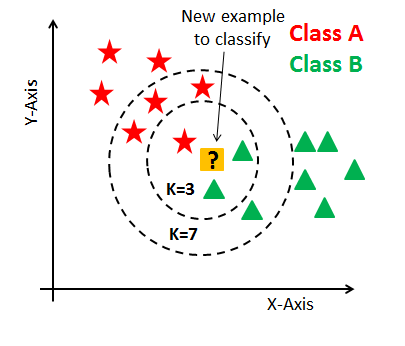
\includegraphics[width=12cm,keepaspectratio]{KNN_final_a1mrv9.png}
  \caption{Schematic of a kNN Classifier's prediction dependency on $k$\cite{knn}. $k=3$ would result in a prediction of class B and $k=7$ would lead to a prediction of class A.}
  \label{fig:knn}
\end{figure}

The $k$ nearest neighbors (kNN) classifier is a classifier that makes its prediction based on the $k$ nearest neighbors of an object. The distance between two objects is measured in the phase space of all considered attributes.
There are a variety of ways to define the distance, but a simple possibility would be the euclidian distance.
The training of the classifier solely consists of saving the training data.
The classifiction principle is depicted in \autoref{fig:knn}.
An object is classified as the class, which the majority of the $k$ nearest neighbors are in.

The prediction is highly dependent on the choice of$k$. kNN Classifiers with low $k$ are sensitive to statistical fluctuations and those with high $k$ can have worse predictions, because they include objects that are really far away. The latter is especially a problem when the training data is sparse or not distributed uniformly.

\subsubsection*{Random Forest Classifier}
The random forest classifier is based on the binary decision tree.
A decision tree consists of nodes at which a cut on one attribute is performed splitting the data. For each node the best split is determined from a random subset of $k$ attributes.
This is done subsequently until a specified depth is reached or if a node only contains one class which is then called a leaf. To prevent overfitting the mean value of a variety of trees is calculated. In a common implementation each tree is trained on a subset of the whole data. The confidence
\begin{equation*}
  c  = \frac{1}{N} \sum\limits_{i=1}^{N} P_i \, , P_i \in \{0,1\}
\end{equation*}
of the prediction then is the arithmetic mean of the decisions $P_i$ of the single trees.

\subsection{Quality Parameters}
The quality of separation of two classes can be evaluated with a variety of quality parameters. A common measure are the
\begin{align*}
  \mathrm{purity}\ p = \frac{tp}{tp + fp} \\
  \mathrm{efficiency} \ r = \frac{tp}{tp + fn}\, .
\end{align*}
Here $tp$ denotes the number of \textit{true positive} predictions, i.e. correctly predicted as signal, wheres $tn$ and $fn$ denote the number of  \textit{true negative} and \textit{false negative} predictions, i.e. correctly and falsely, respectively, predicted background events.\\

To estimate an error for these parameters so called cross validation is used. here the data is split into $n$ subsets of which $n - 1$ are used for training and the remaining is used for validation. This is done $n$ times so that each subset is used as validation set. For each iteration the quality parameters above are calculated and a mean value and standard deviation on these can be given.\\

Another common measure of the quality of binary classifiers are receiver operating characteristics (ROC) curves which show the ratio of true positives or true positive rate ($tpr$) against the ratio of false positives or false positive rate ($fpr$).
A perfect classification would result in a horizontal line at $tpr = 1$ while a totally random classification can be depicted as a diagonal line from $(0,0)$ to $(1,1)$ meaning equally many false positves and true positives would be predicted. The quality of the ROC curve can be described via the area under curve (AUC) score.
Totally random classification would give $\mathrm{AUC} = 0.5$ while a perfect classifier would score $\mathrm{AUC} = 1$.
